\documentclass[a4paper, 12pt]{article}
\usepackage{geometry}
\geometry{margin=2cm}
\usepackage{graphicx} % Required for the inclusion of images
\usepackage[utf8]{inputenc}
%\usepackage{natbib} % Required to change bibliography style to APA
\usepackage{amsmath} % Required for some math elements 
\usepackage[spanish]{babel} 
%\usepackage{fontspec}
\usepackage{lineno,hyperref}
\usepackage{upgreek}
\usepackage{gensymb}
\usepackage{textcomp}
\usepackage{amssymb}
\usepackage{textgreek}
\usepackage{float}
\usepackage{fancyhdr}
\usepackage{dirtytalk}

\allowdisplaybreaks
%\textwidth18cm
%\textheight22cm
%\topmargin0cm
%\oddsidemargin2cm
%\hypersetup{hidelinks}

\usepackage{multirow}

\hypersetup{
    colorlinks=true,
    linkcolor=blue,
    }
\graphicspath{{img}}
\setlength\parindent{0pt} % Removes all indentation from paragraphs

\renewcommand{\labelenumi}{\alph{enumi}.} % Make numbering in the enumerate environment by letter rather than number (e.g. section 6)

\renewcommand{\b}{\textbf}

\newsavebox{\mygraphic}
\sbox{\mygraphic}{
\includegraphics[height=1cm]{logoUNRN.jpg}}


\pagestyle{fancy}

\fancyhead{}

\headheight 16pt

\fancyhead[LO]{\setlength{\unitlength}{1in}
	\begin{picture}(0,0)
		\put(0,0){\usebox{\mygraphic}}
	\end{picture}
	\hspace{1cm}
}

\fancyhead[CO] {\hspace{1.5cm} \large Física I: Ingenierías Ambiental, Electrónica y Telecomunicaciones}

%esto me pareció piola para enumerar los ejercicios
%lo saqué de acá: https://tex.stackexchange.com/questions/302948/numbered-exercises-as-sections
%%%%%%%%%%%%%%%%%%%%%%%%%%%%%%%%%%%%%%%%%5
\newcounter{eje}
\setcounter{eje}{0}
\newcounter{subeje}
\setcounter{subeje}{-1}
\renewcommand\thesubeje{\arabic{eje}\alph{subeje}}%
\newcommand \eje{%
  \vspace{.2cm}
  \par\noindent
  \ifnum\value{subeje}>-1
    \refstepcounter{subeje}%
    \llap{\thesubeje)\quad}%
  \else
    \refstepcounter{eje}%
    \llap{\theeje)\quad}%
  \fi
}
\begin{document}
\pagestyle{fancy}

\begin{center}

	{\Large \textbf{Tercer parcial}}
 
\vspace{.2cm}

{viernes 10/11}
\end{center}

Tome para el valor de g = 9.8 m/s$^2$.

\eje{\bf TEMA 7: ELASTICIDAD} Se cuelga una viga de 2 t de dos cables de la misma sección, uno de aluminio y otro de acero. Al suspenderla, ambos cables se estiran lo mismo. Calcular la tensión que soporta cada uno. Módulos de Young: acero = $20\times 10^{10}$ N/m$^2$, aluminio = $7\times 10^{10}$ N/m$^2$.

\begin{figure}[H]
\begin{center}
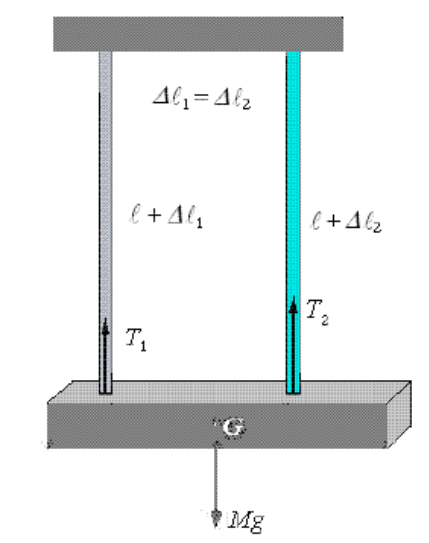
\includegraphics[clip,width = .45\columnwidth]{img/3erparcial2023-2.png}
\end{center}
\end{figure}

\vspace{-0.5cm}

\eje{\bf TEMA 8: ONDAS} 

a) Dos trenes se mueven uno hacia el otro a una velocidad de 90 km/h relativa al suelo. Si uno de los trenes emite una señal a 520 Hz, encuentre la frecuencia que escucharía un pasajero en el otro tren. Use como velocidad el sonido: 340 m/s. 

b) Escriba la ecuación de una onda viajera $y=A\sin{\left(kx-\omega t\right)}$ sabiendo que su velocidad es de 24 m/s, se traslada hacia la derecha (+x) y su representación gráfica a $t=0$ es la de la figura adjunta. 

\begin{figure}[H]
\begin{center}
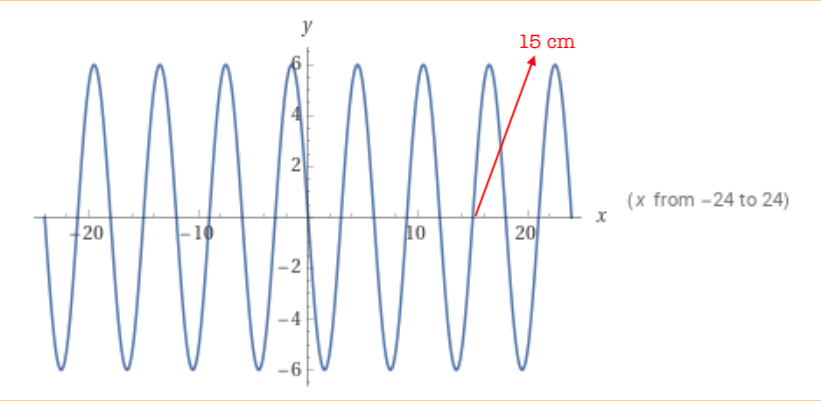
\includegraphics[clip,width = .65\columnwidth]{img/3erparcial2023-1.png}
\end{center}
\end{figure}

\newpage

\eje{\bf TEMA 9: HIDROSTÁTICA E HIDRODINÁMICA} El agua corre por un ca\~no horizontal cuya sección transversal es variable. El ca\~no tiene dos tubos que están fijados verticalmente al ca\~no, como se indica en la figura adjunta, el primero por sobre la sección $A_1$ y el segundo, por sobre la $A_2$. Los tubos verticales permiten observar la diferencia de altura $\Delta h$ que hay entre las columnas de agua que llenan los tubos verticales. 

a) Obtenga la siguiente expresión para el caudal Q: $A_1 A_2\sqrt{\frac{2g\Delta h}{A^2_2-A^2_1}}$

\begin{figure}[H]
\begin{center}
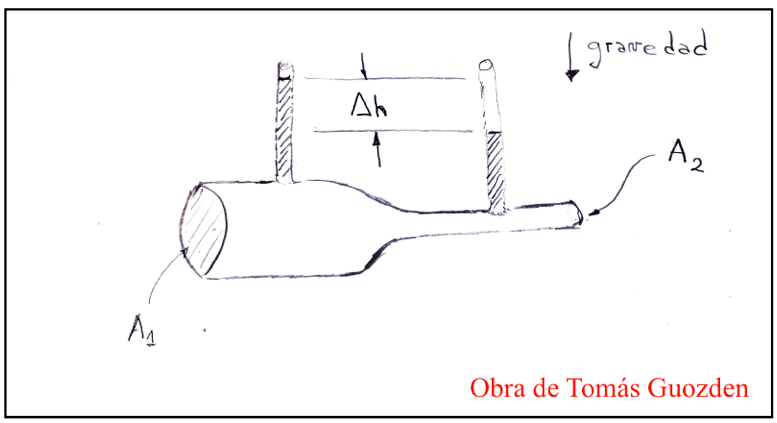
\includegraphics[clip,width = .65\columnwidth]{img/3erparcial2023-0.png}
\end{center}
\end{figure}

\vspace{-0.5cm}
\end{document}